\documentclass[margin=5mm, varwidth]{standalone}
\usepackage[paperwidth=9in,top=1in,bottom=1in,right=1in,left=1in,heightrounded]{geometry}
\usepackage{niftydiags}

\begin{document}
\begin{pycode}
import numpy as np
def rad(deg):
    return deg * np.pi / 180
def roundCoord(point):
    return [ round(x, 2) for x in point ]
def tuplefy(points):
    return ( tuple(roundCoord(p)) for p in points)
\end{pycode}

\section{(Excursion) vector components as linear combinations of vectors.} 

\items{
\item Every vector can be written as a combination of scalars and unit vectors
\item $\vec{v} = \vektor{a\\b} = a \cdot \vektor{1\\0} + b \cdot \vektor{0\\1}$
\item $\hat{e}_1 = \vektor{1\\0}$ and $\hat{e}_2 = \vektor{0\\1}$ are canonical base vectors in $R^2$ \\
      For $R^n$: $\hat{e}_i = \vektor{0 \\ \vdots\\ 1 \\ \vdots \\ 0}$ $i$th component being 1 all other 0
\item Generally: $\vec{v} = \vektor{x_1 \\ x_2 \\ \vdots \\ x_n} = \sum\limits_{i=1}^{n}{x_i \cdot e_i}$
\item Points on the unit cirlce (c=1): 
}

\newcommand\cosdiag{0.7071}
\newcommand\lenax{1.2}
\begin{tikzpicture}[scale=2]
\coordinate (A) at (0, 0);
\coordinate (B) at (\cosdiag, 0);
\coordinate (C) at (\cosdiag, \cosdiag);

\draw[very thin, <->] (-\lenax, 0) -- (\lenax, 0) node[right] {$x$};
\draw[very thin, <->] (0, -\lenax) -- (0, \lenax) node[above]{$y$};
\draw[dashed] (0,0) circle (1);

\newcommand\rad{0.35}
\draw[fill=green!30, very thin] (0,0) -- (45:\rad) arc (45:0:\rad);
\draw (0.22, 0.09) node {$\alpha$};

\newcommand\ninetyrad{\rad /2}
\draw[very thin] (\cosdiag,\ninetyrad) arc (90:180:\ninetyrad);
\fill(\cosdiag - \ninetyrad / 2.5, \ninetyrad / 2.5) circle (0.02);

\draw (A) -- (B) node[midway, below] {$a$};
\draw (B) -- (C) node[midway, right] {$b$} node[above, right] {$\vec{v}$};
\draw (C) -- (A) node[midway, above left] {$c$};
\end{tikzpicture}
\begin{pycode}
deg=0
rotdeg=45
v=(np.cos(rad(deg)), np.sin(rad(deg)) )
v2=(-v[1],v[0])
a=np.multiply(np.cos(rad(rotdeg)), v)
b=np.multiply(np.sin(rad(rotdeg)), v2)
v3=a+b
alphaLoc = np.multiply(0.3, ( np.cos(rad(deg+rotdeg/2)), np.sin(rad(deg+rotdeg/2)) ) )
a, b, v3, alphaLoc = tuplefy([a, b, v3, alphaLoc])
\end{pycode}
\begin{pysub}
    \begin{tikzpicture}[scale=2]
        \coordinate (O) at (0, 0);
        \coordinate (A) at !{v};
        \coordinate (B) at !{v2};
        \coordinate (C) at !{v3};
        \draw[very thin, <->] (-\lenax, 0) -- (\lenax, 0) node[right] {$x$};
        \draw[very thin, <->] (0, -\lenax) -- (0, \lenax) node[above]{$y$};
        \draw[dashed, very thin] (0,0) circle (1);

        \draw[fill=green!30, very thin] (0,0) -- (!{deg}:0.4) arc (!{deg}:!{deg}+!{rotdeg}:0.4);
        \draw !{alphaLoc} node {$\alpha$};
        
        \draw[-latex, thick] (O) -- +(A) node[right, below] {$\hat{e}_1$};
        \draw[-latex, dashed, thick] (O) -- +(B) node[above, left] {$\hat{e}_2$};
        \draw[-latex, dashed, thick] (O) -- +(C) node[right] {$\vec{v}$};

        \draw[dashed, very thin] !{b} -- +!{a};
        \draw[dashed, very thin] !{a} -- +!{b};

        \draw[-latex, thick] (O) -- +!{a} node[midway, below] {$\cos(\alpha) \, \hat{e}_1$};
        \draw[-latex, thick] (O) -- +!{b} node[midway, left] {$\sin(\alpha) \, \hat{e}_2$};
    \end{tikzpicture}
\end{pysub}
\items{
\item $\vec{v} = \vektor{a\\b} = \vektor{\cos(\alpha)\\ \sin(\alpha)} = \cos(\alpha) \cdot \vektor{1\\0} +\sin(\alpha) \cdot \vektor{0\\1} = \cos(\alpha) \cdot \hat{e}_1 +\sin(\alpha) \cdot \hat{e}_2$
}
\section{(Excursion) Orthogonal complement of a vector ($90^\circ$ Rotation CCW)}
\items{
\item Set up orthogonal vector to obtain up-vector for new coordinate frame
}
{ \large
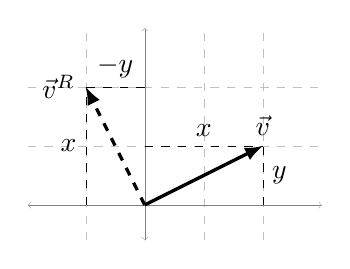
\begin{tikzpicture}[scale=1.5, ultra thin]
\draw[step=0.5cm, dashed, lightgray] (-.99,-0.3) grid (1.49, 1.49);
\draw[<->, gray] (0, -0.3) -- (0, 1.5cm);
\draw[<->, gray] (-0.99, 0) -- (1.5cm, 0);
\draw[very thick, -latex] (0, 0) -- (1, 0.5) node[above] {$\vec{v}$};% = \begin{pmatrix} x \\ y\end{pmatrix}$};
\draw[dashed] (0, .5) -- (1, .5) node[midway, above] {$x$};
\draw[dashed] (1, 0) -- (1, .5) node[midway, right] {$y$};
\draw[very thick, dashed, -latex] (0, 0) -- (-0.5, 1) node[left] {$\vec{v}^{R}$};
\draw[dashed] (0, 1) -- (-.5, 1) node[midway, above] {$-y$};
\draw[dashed] (-.5, 0) -- (-.5, 1) node[midway, left] {$x$};
\end{tikzpicture} }
$\vec{v}^{R} =  \vektor{x\\y} ^{R} = \vektor{-y\\x}$
\\
\items{
\item Derive $\vec{v}^R$: \\ 
$\gleichung{
    \vec{v}^{R}&=&  \vektor{x \\ y} ^{R}= \vektor{\cos(\alpha) \\ \sin(\alpha)} ^{R}=\vektor{ \cos(\alpha + 90^\circ) \\ \sin(\alpha + 90^\circ) }
    \\
    &=& \vektor{ \cos(\alpha) \cos(90^\circ) - \sin(\alpha) \sin(90^\circ)  \\ \cos(\alpha) \sin(90^\circ) + \sin(\alpha) \cos(90^\circ) }
    \\
    &=&\vektor{ \cos(\alpha) \cdot 0 - \sin(\alpha) \cdot 1   \\ \cos(\alpha) \cdot 1 + \sin(\alpha) \cdot 0 }
    = \vektor{ - \sin(\alpha) \\ \cos(\alpha) } = \underline{\vektor{- y \\ x }}
}$
\item $\vec{v}^{R}$ is perpendicular to $\vec{v}$: $ \vektor{x \\ y} \bullet \vektor{-y \\ x} = \underline{-xy + yx = 0}$
}

\section{From 2D vector arithmetic to 2D rotation matrix}

\items {
\item Apply $\cos$ and $\sin$ to new coordinate frame with axes $\vec{v}$ and $\vec{v}^R$ to obtain rotated vector $\vec{v}'$
}

\begin{pycode}
deg=25
rotdeg=45
v=(np.cos(rad(deg)), np.sin(rad(deg)) )
v2=(-v[1],v[0])
a=np.multiply(np.cos(rad(rotdeg)), v)
b=np.multiply(np.sin(rad(rotdeg)), v2)
v3=a+b
alphaLoc = np.multiply(0.3, ( np.cos(rad(deg+rotdeg/2)), np.sin(rad(deg+rotdeg/2)) ) )
a, b, v3, alphaLoc = tuplefy([a, b, v3, alphaLoc])
\end{pycode}
\begin{pysub}
    \begin{tikzpicture}[scale=2]
        \coordinate (O) at (0, 0);
        \coordinate (A) at !{v};
        \coordinate (B) at !{v2};
        \coordinate (C) at !{v3};
        \draw[very thin, <->] (-\lenax, 0) -- (\lenax, 0) node[right] {$x$};
        \draw[very thin, <->] (0, -\lenax) -- (0, \lenax) node[above]{$y$};
        \draw[dashed, very thin] (0,0) circle (1);

        \draw[fill=green!30, very thin] (0,0) -- (!{deg}:0.4) arc (!{deg}:!{deg}+!{rotdeg}:0.4);
        \draw !{alphaLoc} node {$\alpha$};
        
        \draw[-latex, thick] (O) -- +(A) node[above] {$\vec{v}$};
        \draw[-latex, dashed, thick] (O) -- +(B) node[above] {$\vec{v}^{R}$};
        \draw[-latex, dashed, thick] (O) -- +(C) node[above] {$\vec{v}'$};

        \draw[dashed, very thin] !{b} -- +!{a};
        \draw[dashed, very thin] !{a} -- +!{b};

        \draw[-latex, thick] (O) -- +!{a} node[midway, right] {$\cos(\alpha) \, \vec{v}$};
        \draw[-latex, thick] (O) -- +!{b} node[midway, left] {$\sin(\alpha) \, \vec{v}^{R}$};
    \end{tikzpicture}
\end{pysub}

\items {
\item $\vec{v}' = \cos(\alpha) \, \vec{v} + \sin(\alpha) \, \vec{v}^{R}$
\item rearrange to matrix arithmetic to apply transformation to arbitrary vector \\
$\gleichung{
    v' &=& \cos(\alpha) \, \vektor{x \\ y}  + \sin(\alpha) \, \vektor{-y \\ x} 
    &=& \vektor{\cos(\alpha) \, x \\ \cos(\alpha) \, y}  + \vektor{ -\sin(\alpha) \, y \\ \sin(\alpha) \, x} 
    \\
    &=& \vektor{\cos(\alpha) \, x  -\sin(\alpha) \, y \\ \sin(\alpha) \, x + \cos(\alpha) \, y} 
    &=& \underline{\mymat{\cos(\alpha) \, & -\sin(\alpha) \, \\ \sin(\alpha) \, & \cos(\alpha) \,} } \, \vektor{x \\ y}
}$
}

\section{3D Angle-Axis Rotation(Rodrigues' rotation formula)}

\items{
\item Set up parametric plane equation placed orthogonal to rotation axis(normal) and rotate vector along plane. \\  
\item Points (x,y) on plane P (${R^3}$): \\ $P(x, y) =  \vec{c} + x \, \vec{a} +  y \, \vec{b}$ with $\vec{a} \bullet \vec{b} = 0$ \\ 
Circle on plane: $P(\cos(\theta), \sin(\theta)) =  \vec{c} + \cos(\theta) \, \vec{a} +  \sin(\theta) \, \vec{b}$ 
}

\newcommand\unit{.8}
\newcommand\hgt{.6}
\newcommand\myscale{4}	
\begin{tikzpicture}[scale=\myscale, x={({cos(20)},{-sin(20)},0)},z={({-sin(40)},{-cos(40)},0)}]
    \draw[dashed] (-\unit/2,\hgt,\unit/2) -- (-\unit/2,\hgt,-\unit/2) -- (\unit/2,\hgt,-\unit/2) -- (\unit/2,\hgt,\unit/2) -- cycle;
%    \draw[-latex] (0,0,0) -- (0, 1, 0) node[above] {$\hat{n}$};
%    \draw[-latex] (0,0,0) -- (.4, .6, 0) ;%node[right] {$\vec{v}$};
    \draw[-latex] (0, .6, 0) -- (.4, .6, 0) node[midway, above right] {$\vec{a}$};
    \draw[-latex] (0, 0.6, 0) -- (0, 0.6, -.4) node[above right] {$\vec{b}$};
    \draw[-latex] (0, 0, 0) -- (0, .6, 0) node [below left] {$\vec{c}$};
\end{tikzpicture}
\begin{tikzpicture}[scale=\myscale, x={({cos(20)},{-sin(20)},0)},z={({-sin(40)},{-cos(40)},0)}]
%    \draw[-latex, very thick] (0,0,0) -- (0, 1, 0) node[above] {$\hat{n}$};
%    \draw[-latex] (0,0,0) -- (.4, .6, 0);% node[right] {$\vec{v}$};
    \newcommand\rad{.4}
    \draw[fill=green!30, dashed] (\rad, \hgt, 0) \foreach \X in {0,-5,...,-45} { -- ({\rad/2*cos(\X)},\hgt,{\rad/2*sin(\X)}) } --  (0, \hgt, 0);
    \draw[dashed] (\rad, \hgt, 0) \foreach \X in {0,10,...,360} { -- ({\rad*cos(\X)},\hgt,{\rad*sin(\X)}) };

    \draw[-latex] (0, .6, 0) -- (.4, .6, 0) node[below] {$\vec{a}$};
    \draw[-latex] (0, 0.6, 0) -- (0, 0.6, -.4) node[above right] {$\vec{b}$};
    \draw[-latex] (0, 0, 0) -- (0, .6, 0) node [below left] {$\vec{c}$};

    \draw[-latex, dashed] (0, .6, 0) -- ({.4*cos(-45)}, .6, {.4*sin(-45)}) node[above right] {$P(\cos(\theta),\sin(\theta))$};

    \draw[dashed] (0, .6, {.4*sin(-45)}) -- ({.4*cos(-45)}, .6, {.4*sin(-45)});
    \draw[dashed] ({.4*cos(-45)}, .6, 0) -- ({.4*cos(-45)}, .6, {.4*sin(-45)});
    \draw[-latex, thick] (0, .6, 0) -- (0, .6, {.4*sin(-45)}) node[midway, left] {$\sin(\theta) \, \vec{b}$};
    \draw[-latex, thick] (0, .6, 0) -- ({.4*cos(-45)}, .6, 0) node[midway, below] {$\cos(\theta) \, \vec{a}$};

%    \draw[dashed] (0, .6, 0) node {};
%    \draw[dashed] (0, .6, 0)node {};

    \draw (0.15, \hgt ,-0.05) node []{$\theta$};
\end{tikzpicture}

\items{
    \item With $\hat{n}$ rotation axis and normal to the plane of rotation\\ 
    { \small(the rotation axis vector $\hat{n}$ needs to be normalized, because of the projection operation)}
    \item $\vec{v}$ vector to be rotated around axis vector $\hat{n}$
    \item Construct plane of rotation with rejection(projection) of $\vec{v}$ onto $\hat{n}$ and cross product of $\vec{n}$ with $\hat{v}$
}

\begin{tikzpicture}[scale=\myscale, x={({cos(20)},{-sin(20)},0)},z={({-sin(40)},{-cos(40)},0)}]
    \newcommand\rad{.25}
    \draw[-latex, very thick] (0,0,0) -- (0, 1, 0) node[above] {$\hat{n}$};
    \draw[-latex, very thick] (0,0,0) -- (.4, .6, 0) node[right] {$\vec{v}$};
    \draw (\rad, \hgt, 0) \foreach \X in {0,-5,...,-45} { -- ({\rad*cos(\X)},\hgt,{\rad*sin(\X)}) };
    \draw[dashed] (0, .6, 0) -- (.4, .6, 0);
    \draw[-latex, dashed] (0, .6, 0) -- ({.4*cos(-45)}, .6, {.4*sin(-45)}) node[above] {$\vec{v'}$};
\end{tikzpicture}
\begin{tikzpicture}[scale=\myscale, x={({cos(20)},{-sin(20)},0)},z={({-sin(40)},{-cos(40)},0)}]
    \draw[dashed] (-\unit/2,\hgt,\unit/2) -- (-\unit/2,\hgt,-\unit/2) -- (\unit/2,\hgt,-\unit/2) -- (\unit/2,\hgt,\unit/2) -- cycle;
    \draw[-latex, thick] (0,0,0) -- (0, 1, 0) node[above] {$\hat{n}$};
    \draw[-latex, thick] (0,0,0) -- (.4, .6, 0) node[right] {$\vec{v}$};
    \draw[-latex, dashed] (0, .6, 0) -- (.4, .6, 0) node[midway, above right] {$\vec{a}$};
    \draw[-latex, thick] (0, 0, 0) -- (0, .6, 0) node [below left] {$\vec{c}$};
    \draw[-latex, thick] (0, 0.6, 0) -- (0, 0.6, -.4) node[above right] {$\vec{b}$};
\end{tikzpicture}
\begin{tikzpicture}[scale=\myscale, x={({cos(20)},{-sin(20)},0)},z={({-sin(40)},{-cos(40)},0)}]
    \draw[dashed] (-\unit/2,\hgt,\unit/2) -- (-\unit/2,\hgt,-\unit/2) -- (\unit/2,\hgt,-\unit/2) -- (\unit/2,\hgt,\unit/2) -- cycle;
    \draw[-latex, very thick] (0,0,0) -- (0, 1, 0) node[above] {$\hat{n}$};
    \draw[-latex, very thick] (0,0,0) -- (.4, .6, 0) node[right] {$\vec{v}$};
    \draw[-latex, dashed] (0, .6, 0) -- (.4, .6, 0) node[midway, above right] {$\vec{v}_{\perp}$};
    \draw[-latex,  thick] (0, 0, 0) -- (0, .6, 0) node [below left] {$\vec{v}_{\parallel}$};
    \draw[-latex,  thick] (0, 0.6, 0) -- (0, 0.6, -.4) node[above right] {$\hat{n} \times \vec{v}$};
\end{tikzpicture}
\begin{tikzpicture}[scale=\myscale, x={({cos(20)},{-sin(20)},0)},z={({-sin(40)},{-cos(40)},0)}]
    \draw[-latex, very thick] (0,0,0) -- (0, 1, 0) node[above] {$\hat{n}$};
    \draw[-latex, very thick] (0,0,0) -- (.4, .6, 0) node[right] {$\vec{v}$};
    \draw[-latex, dashed] (0, .6, 0) -- (.4, .6, 0) node[midway, above] {$\cos_\theta \vec{v}_{\perp}$};
    \draw[-latex,  thick] (0, 0, 0) -- (0, .6, 0) node [below left] {$\vec{v}_{\parallel}$};
    \draw[-latex,  thick] (0, 0.6, 0) -- (0, 0.6, -.4) node[above right] {$\sin_\theta \hat{n} \times \vec{v}$};
    \newcommand\rad{.4}
    \draw[dashed] (\rad, \hgt, 0) \foreach \X in {0,10,...,360} { -- ({\rad*cos(\X)},\hgt,{\rad*sin(\X)}) };
\end{tikzpicture}

\items{
\item $\vec{v} = \vec{v_\perp} + \vec{v_\parallel}$
\item $\vec{v}_\parallel$ part of $\vec{v}$ parallel to $\hat{n}$ (Projection of $\vec{v}$ onto $\hat{n}$)\\
      $\vec{c} \rightarrow \vec{v_\parallel} = ( \hat{n} \bullet \vec{v} ) \hat{n}$ 
\item $\vec{v}_\perp$ part of $\vec{v}$ perpendicular to $\hat{n}$ \\
      $\vec{a} \rightarrow \vec{v_\perp} = \vec{v} - \vec{v_\parallel} = \vec{v} - ( \hat{n}\bullet \vec{v}) \hat{n}$
\item vector in plane perpendicular to $\vec{v}$ and $\hat{n}$\\
      $\vec{b} \rightarrow \hat{n} \times \vec{v} = \hat{n} \times \vec{v}_\perp $ \\
\item $\vec{v'} = \vec{v}_\parallel + \cos_\theta \, \vec{v}_\perp + \sin_\theta \, \hat{n} \times \vec{v}$
}

\subsection{Derivation of Rodrigues Rotation Matrix:}

\items{

\item Express vector arithmetic terms with matrix arthimic equivalents: \\
{ \small(Generally you can convert any vector arithmetic terms by transforming the base vectors of a space or the column vectors of a matrix. In case of the projection of a vector we can rearrange the operation to get it directly) }

\item[]

\item $\mathbf{K}$ is skew symmetric matrix which can used calculate the cross product of $\hat{n}$ with $\vec{v}$: \\
$\mathbf{K} \, \vec{v} = \hat{n} \times \vec{v} = [\hat{n}]_{\times} \, \vec{v}$ \\
$\mathbf{K} = [\hat{n}]_{\times} = \mymat{&&\\ \hat{n}\times\hat{e}_1 & \hat{n}\times\hat{e}_2 & \hat{n}\times\hat{e}_3 \\ && } \\
= 
\mymat{
\vektor{ n_y \cdot 0 - n_z \cdot 0 \\ n_z \cdot 1 - n_x \cdot 0 \\ n_x \cdot 0 - n_y \cdot 1 } & 
\vektor{ n_y \cdot 0 - n_z \cdot 1 \\ n_z \cdot 0 - n_x \cdot 0 \\ n_x \cdot 1 - n_y \cdot 0 } &
\vektor{ n_y \cdot 1 - n_z \cdot 0 \\ n_z \cdot 0 - n_x \cdot 1 \\ n_x \cdot 0 - n_y \cdot 0 } 
}
=
\mymat{ 0 & -n_z & n_y \\ n_z & 0 & -n_x \\ -n_y & n_x & 0 } $

\item[]

\item $\mathbf{P}$ is the matrix which multiplied with projects a vector $\vec{v}$ onto normal $\hat{n}$:\\
$\mathbf{P} \, \vec{v} = (\vec{v} \bullet \hat{n}) \, \hat{n} = (\hat{n} \bullet \vec{v}) \hat{n} = (\hat{n}^T \hat{v})\hat{n} = \hat{n}\hat{n}^T \vec{v} $\\
$\gleichung{
& & \, \mymat { n_x & n_y & n_z } \\
\mathbf{P} = \hat{n} \hat{n}^\textsf{T} =  & \mymat{ n_x \\ n_y \\ n_z } & 
  \mymat { n_x^2 & n_x n_y & n_x n_z  \\
    n_x n_y & n_y^2 & n_y n_z  \\
    n_x n_z & n_y n_z & n_z^2  \\ }
}$

\item[]

\item rearrange vector arithmetic rotation formula to matrix arithmetic (and factorize $\vec{v}$) \\
$\gleichung{
    \vec{v'}
      & = \vec{v}_\parallel + \cos(\theta) \, \vec{v}_\perp + \sin(\theta) \, \hat{n} \times \vec{v} &|& \text{def. } \vec{v}_\parallel, \vec{v}_\perp\\
      & =  (\vec{v} \bullet \hat{n} ) \hat{n} + \cos(\theta) \left(\vec{v} - ( \vec{v} \bullet \hat{n} ) \hat{n} \right) + \sin(\theta) \, \hat{n} \times \vec{v} &|& (\vec{v} \bullet \hat{n}) \hat{n} = (\hat{n}^T \hat{v})\hat{n} = \hat{n}\hat{n}^T \vec{v}\\
      & =  \hat{n}\hat{n}^{T} \vec{v} + \cos(\theta) \left(\vec{v} - \hat{n}\hat{n}^{T} \vec{v} \right) + \sin(\theta) \, [\hat{n}]_{\times} \vec{v} &|& \mathbf{P} = \hat{n}\hat{n}^T, \mathbf{K} = [\hat{n}]_\times, \mathbf{I} \, \vec{v} = \vec{v} \\
      & =  \mathbf{P} \, \vec{v} + \cos(\theta) \left(\mathbf{I} \, \vec{v} - \mathbf{P} \, \vec{v} \right) + \sin(\theta) \, \mathbf{K} \, \vec{v} &|& \text{factorize } \vec{v}: \mathbf{A} \vec{v} + \mathbf{B} \vec{v} = [ \mathbf{A} + \mathbf{B} ] \vec{v} \\
      & =  [\, \mathbf{P} + \cos(\theta) \left(\mathbf{I} - \mathbf{P} \right) + \sin(\theta) \, \mathbf{K} \, ] \, \vec{v} \\
      & = \mathbf{R}(\hat{n}, \theta) \, \vec{v}
    }$

\item[]

\item Matrix for rotating arbitrary vector around axis $\hat{n}$ with angle $\theta$: \\ 
$\mathbf{R}(\hat{n}, \theta) =  \mathbf{P} + \cos(\theta) \left(\mathbf{I} - \mathbf{P} \right) + \sin(\theta) \, \mathbf{K}$ \\

$\mathbf{R}(\hat{n}, \theta) =  \mymat { n_x^2 & n_x n_y & n_x n_z  \\ n_x n_y & n_y^2 & n_y n_z  \\ n_x n_z & n_y n_z & n_z^2  \\ } + \cos(\theta) \left( \mymat{ 1 & 0 & 0 \\ 0 & 1 & 0 \\ 0 & 0 & 1 } - \mymat { n_x^2 & n_x n_y & n_x n_z  \\ n_x n_y & n_y^2 & n_y n_z  \\ n_x n_z & n_y n_z & n_z^2  \\ } \right) + \sin(\theta) \, \mymat{ 0 & -n_z & n_y \\ n_z & 0 & -n_x \\ -n_y & n_x & 0 } $

}

\end{document}
	

%\draw \foreach \X [remember=\X as \lastX (initially 0)] in {0,10,...,360} { ({\unit*cos(\lastX)},0,{\unit*sin(\lastX)}) -- ({\unit*cos(\X)},0,{\unit*sin(\X)}) };

